\chapter{LiDARと不可視情報を統合したMulti MCLと位置推定切り替えシステム}
\label{cha:simulation_experiments}
\graphicspath{{figures/06}}
\section{LiDARと磁気，Wi-Fi情報を統合したMulti MCL}
\section{位置推定切り替えシステム}
\section{自己位置推定の実験}
\subsection{実験方法}
本研究では，開発したMag MCL，Wi-Fi MCLと従来手法を比較するとともに，
車や自転車などの幾何情報が変化する環境における提案手法の有効性を検証する．
実験は宇都宮大学陽東キャンパスの敷地内で実施し，\cref{fig:path}の2つの経路で評価を行った．
Path 2に含まれる駐車場および駐輪場では，車，自転車および太陽光パネルを含む環境で幾何地図を作成した後，
これらの物体を地図上から意図的に削除した．
実験時にはこれらの物体が実際に存在する状態で走行することで，
地図と実環境の幾何情報が異なる状況を再現した．
実験方法は，ロボットが地図作成のための経路と実験用の経路を走行し，磁気強度，オドメトリ，LiDARによる
点群情報，そしてWi-Fi強度情報をrosbagに記録した．
その後，rosbagから幾何地図，磁気地図，Wi-Fi地図を作成した．
最後に，実験用のrosbagからLiDAR MCL（ESS＝1.0）と提案手法の比較を行った．
Wi-Fi MCLのESSの閾値は0.99，その他の手法の閾値は0.9，パーティクル数は1000個とし，
磁気地図および屋外地図のグリッドサイズは0.2[m]，Wi-Fi地図は1.0[m]とした．
また位置推定切り替えシステムの各閾値は，LiDAR平均尤度は0.2，Wi-Fi電波強度平均尤度は0.0085，磁気強度平均尤度は2.0，95\%誤差楕円の長軸半径は2.0[m]とした．

\begin{figure}[tb]
  \centering
  \begin{subfigure}[t]{0.4\columnwidth}
    \centering
    \includegraphics[width=\linewidth]{Path1.png}
    \caption{Path1}
    \label{fig:path1}
  \end{subfigure}
  \hfill
  \begin{subfigure}[t]{0.4\columnwidth}
    \centering
    \includegraphics[width=\linewidth]{Path2.png}
    \caption{Path2}
    \label{fig:Path2}
  \end{subfigure}
  \caption{Path used for Experiment}
  \label{fig:path}
\end{figure}

% 右段に Table 1 -> Table 2 -> Fig. 2 -> Fig. 3 の順で配置
\begin{figure}[!t]
  \centering

  % ==========================================================
  % Table 1: Path 1
  % ==========================================================
\begin{minipage}{\columnwidth}
  \centering
  \captionof{table}{Position and heading errors on Path 1}
  \label{tab:path1_localization_error}
  \scriptsize
  \setlength{\tabcolsep}{3.8pt}
  \renewcommand{\arraystretch}{1.08}
  \small

  \begin{tabular}{lrrrrrr}
    \toprule
    &
    \multicolumn{3}{c}{Position error [m]} &
    \multicolumn{3}{c}{Heading error [deg]} \\
    \cmidrule(lr){2-4}
    \cmidrule(lr){5-7}
    Method &
    MAE & Std. & Max. &
    MAE & Std. & Max. \\
    \midrule
    LiDAR
      & 0.33 & 0.14 & 0.90
      & 0.44 & 0.50 & 9.08 \\
    Multi
      & 0.31 & 0.15 & 0.77
      & 0.45 & 0.46 & 8.76 \\
    Mag
      & 2.34 & 1.46 & 5.59
      & 2.92 & 2.41 & 10.54 \\
    Mag w/o Heading
      & 2.36 & 1.41 & 5.73
      & 3.09 & 2.63 & 15.50 \\
    Wi-Fi
      & 2.48 & 1.17 & 5.63
      & 3.45 & 2.61 & 12.31 \\
    Conventional Wi-Fi
      & 3.06 & 1.71 & 8.77
      & 5.05 & 4.18 & 17.79 \\
    Pose Selector
      & 0.33 & 0.14 & 0.75
      & 0.43 & 0.47 & 9.08 \\
    \bottomrule
  \end{tabular}
\end{minipage}

  \vspace{1.2em}

  % ==========================================================
  % Table 2: Path 2
  % ==========================================================
\begin{minipage}{\columnwidth}
  \centering
  \captionof{table}{Position and heading errors on Path 2}
  \label{tab:path2_localization_error}
  \scriptsize
  \setlength{\tabcolsep}{3.8pt}
  \renewcommand{\arraystretch}{1.08}
  \small

  \begin{tabular}{lrrrrrr}
    \toprule
    &
    \multicolumn{3}{c}{Position error [m]} &
    \multicolumn{3}{c}{Heading error [deg]} \\
    \cmidrule(lr){2-4}
    \cmidrule(lr){5-7}
    Method &
    MAE & Std. & Max. &
    MAE & Std. & Max. \\
    \midrule
    LiDAR
      & 13.28 & 14.72 & 53.47
      & 14.28 & 18.53 & 76.04 \\
    Multi
      & 0.56 & 0.66 & 4.08
      & 1.56 & 2.02 & 13.46 \\
    Mag
      & 1.47 & 0.89 & 5.40
      & 2.51 & 1.98 & 17.56 \\
    Mag w/o Heading
      & 1.59 & 1.00 & 4.24
      & 2.70 & 2.09 & 15.69 \\
    Wi-Fi
      & 2.84 & 1.35 & 7.01
      & 3.17 & 2.37 & 12.60 \\
    Conventional Wi-Fi
      & 3.36 & 1.95 & 10.15
      & 5.56 & 5.45 & 35.53 \\
    Pose Selector
      & 0.56 & 0.66 & 4.08
      & 1.55 & 2.03 & 13.46 \\
    \bottomrule
  \end{tabular}
\end{minipage}

  \vspace{1.2em}

  % ==========================================================
  % Fig. 2: Path 1
  % 図幅は元の 0.7\columnwidth のまま
  % ==========================================================
  \begin{minipage}{\columnwidth}
    \centering
    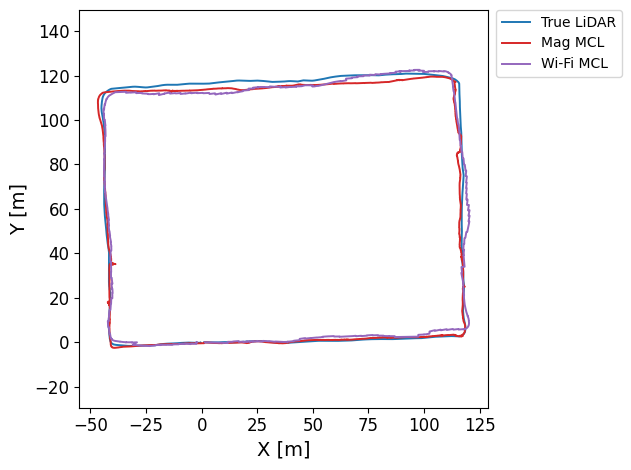
\includegraphics[
      width=0.5\columnwidth
    ]{path1_result.png}
    \captionof{figure}{
      Comparison of localization trajectories on Path 1
    }
    \label{fig:path1_result}
  \end{minipage}

  \vspace{1.2em}

  % ==========================================================
  % Fig. 3: Path 2
  % 図幅は元の 0.7\columnwidth のまま
  % ==========================================================
  \begin{minipage}{\columnwidth}
    \centering
    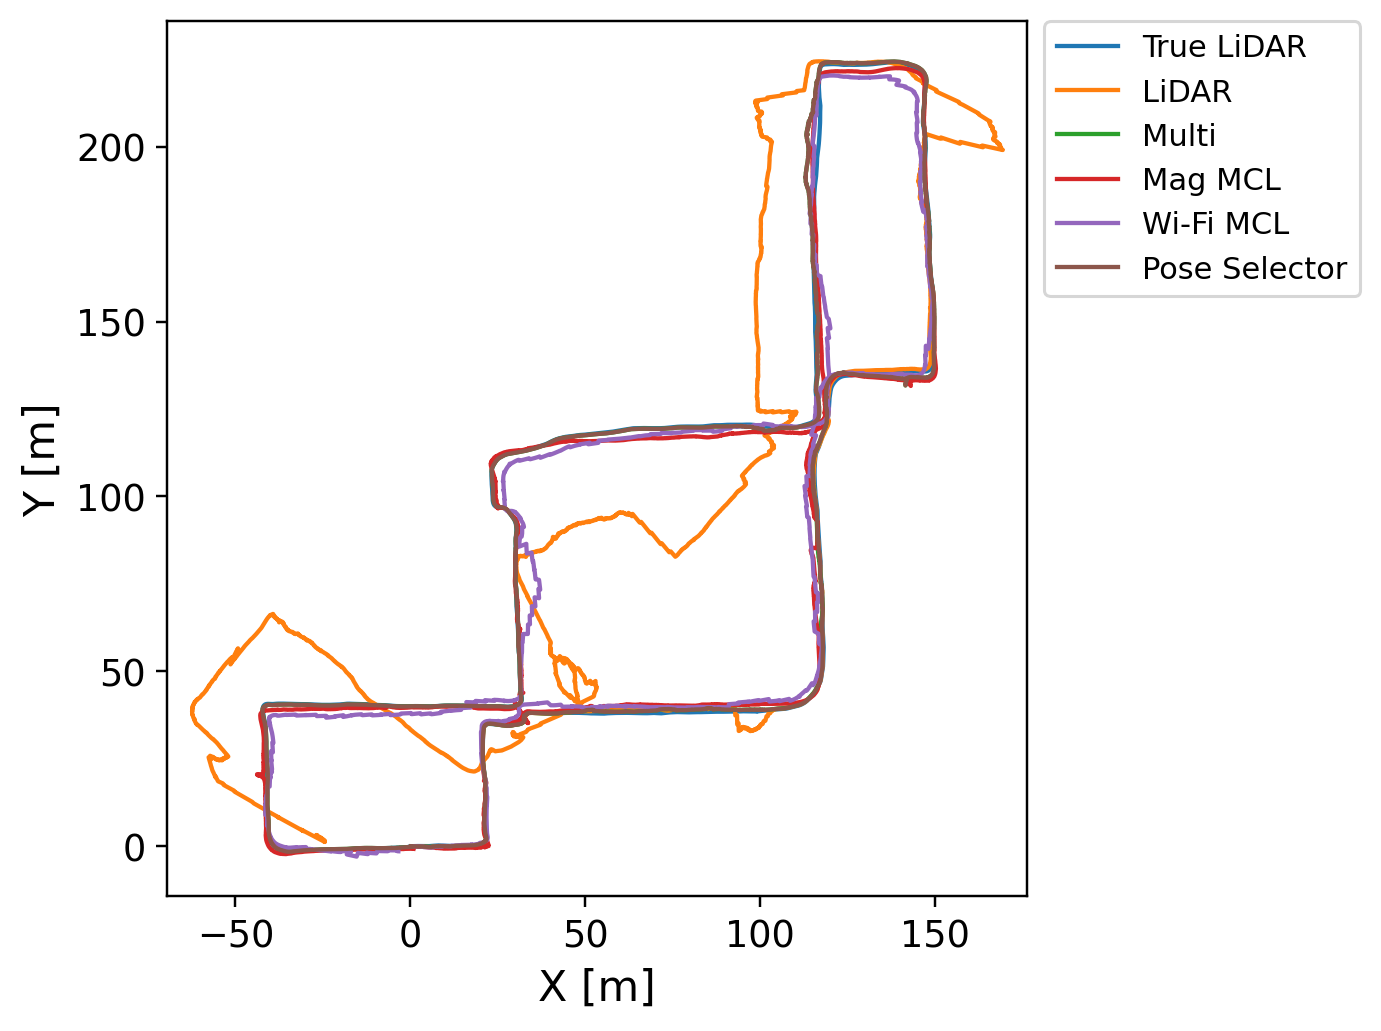
\includegraphics[
      width=0.5\columnwidth
    ]{path2_result.png}
    \captionof{figure}{
      Comparison of localization trajectories on Path 2
    }
    \label{fig:path2_result}
  \end{minipage}

\end{figure}

\subsection{実験結果}
Path 1およびPath 2の実験結果を
\cref{tab:path1_localization_error}および
\cref{tab:path2_localization_error}に，
各自己位置推定手法の推定軌跡を
\cref{fig:path1_result}および
\cref{fig:path2_result}に示す．
\cref{tab:path1_localization_error}，\cref{tab:path2_localization_error}の結果から，
Mag MCLは，方位尤度を使用しない従来のMag MCLと比較して，
位置誤差および角度誤差の最大値は増加したものの，
平均誤差が低減したことから，方位尤度の導入により位置推定精度が
改善された．
次に，Wi-Fi MCLは，Path 1およびPath 2の両方において，
従来手法と比較して位置誤差および角度誤差が低減した．
さらに，\cref{tab:path1_localization_error}および
\cref{tab:path2_localization_error}に示す最大位置誤差それぞれ5.63[m]および7.01[m]であり，
先行研究\cite{akiyama2026wifi}における最大位置誤差9.19[m]を
いずれも下回っていることから，本手法の有効性が確認された．
また，\cref{fig:path2_result}に示すように，
Path 2では，実環境に存在する車両，自転車および太陽光パネルが
幾何地図から削除されているため，
地図とLiDAR観測の間に不一致が生じ，
LiDAR MCLの自己位置推定精度が低下した．
一方，Multi MCLは平均位置誤差が小さく，
真値の軌跡に追従していることから，
異なるセンサ情報を統合することの優位性が確認された．
最後に，LiDAR MCLの失敗検知システムでは，\cref{fig:priority}から位置推定信頼度が低下した区間において，
選択する自己位置推定がLiDAR MCLからMulti MCLへ切り替わった．
このことから，幾何情報の変化によりLiDARに基づく位置推定精度が低下する環境において，
提案した自己位置推定切替システムの有効性が確認された．

\begin{figure}[tb]
  \centering
  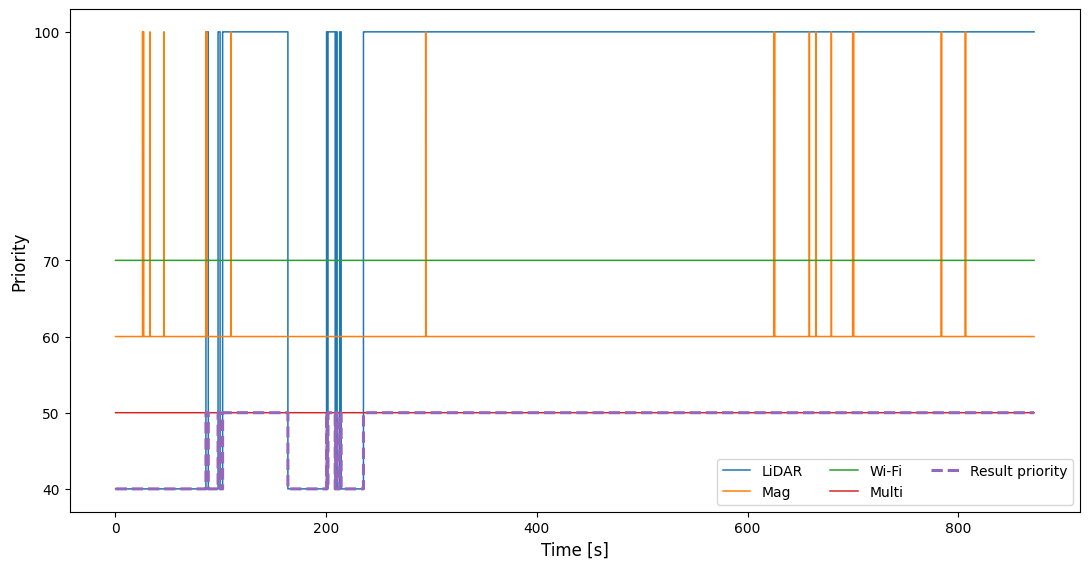
\includegraphics[
    width=0.5\columnwidth
  ]{priority.png}
  \caption{
    Temporal changes in the priority values of each localization method
    and the pose selector on Path 2
  }
  \label{fig:priority}
\end{figure}

\section{考察}
実験結果から本研究で開発したMag MCL，Wi-Fi MCLは真値の軌跡に追従し，自己位置推定ができていることがわかる．
\cref{fig:mahalanobis_result}に，
各時刻における真値とMag MCLおよびWi-Fi MCLの
パーティクル分布との二乗マハラノビス距離の分布を示す．
Mag MCLでは，Path 1において95\%誤差楕円外となった割合は1.79\%，
99\%誤差楕円外となった割合は0.74\%であった．
一方，Path 2では95\%誤差楕円外となった割合は0.055\%であり，
99\%誤差楕円外となるデータ点は確認されなかった．
Wi-Fi MCLでは，Path 1における95\%誤差楕円外となった割合は2.06\%であり，
99\%誤差楕円外となるデータ点は確認されなかった．
また，Path 2では95\%および99\%誤差楕円外となる
データ点は確認されなかった．
以上より，Mag MCLおよびWi-Fi MCLは，
大部分の区間で真値付近のパーティクルを保持していたと推察できる．
したがって，LiDAR MCLの優先度が低下した際に，
これらのパーティクル分布を利用することで，
自己位置推定の復帰に有効なパーティクルをサンプリングできる可能性がある．

次に，位置推定切り替えシステムについて考察する．
\cref{tab:lidar_failure_detection}に，
Path 2におけるLiDAR MCLの失敗検知の性能を，
適合率（Precision），再現率（Recall）および
偽陽性率（FPR）を用いて評価した結果を示す．
本研究では，高精度な位置推定手法であるLiDAR MCLにおいて，
位置誤差が1[m]以上となった状態を推定失敗として扱った．
LiDAR平均尤度およびパーティクル分布の広がりを用いた判定は，
再現率が高く，多くの推定失敗を検出できた．
一方で，適合率が比較的低く，偽陽性率が高いことから，
LiDAR MCLが正しい位置を推定している場合にも，
誤って失敗と判定される可能性がある．
また，これらのLiDAR情報のみに基づく指標では，
幾何構造が類似した場所に誤収束した場合に，
推定失敗を検出できない可能性がある．
一方，LiDAR MCLの推定位置が
Wi-Fi MCLおよびMag MCLの推定分布内に存在するかを評価する指標と，
LiDAR MCLのパーティクルに対するWi-Fi平均尤度を用いた指標は，
再現率は他の指標より低いものの，
適合率が高く，偽陽性率が低い結果となった．
したがって，これらの指標は検出可能な失敗が限定される一方で，
正常な位置推定を失敗と誤判定する可能性が低く，
信頼性の高い判定指標であると考察できる．
このことから，提案した指標を組み合わせて位置推定手法を切り替えることは，
ロバストな自己位置推定に有効である．

最後に，Multi MCLは，
幾何情報が変化する環境においても高い位置推定精度を示した．
しかし，位置誤差が2\sim 4[m]程度となった区間では，
真値がMulti MCLの99\%誤差楕円外となる場合が確認された．
Multi MCLではLiDAR尤度も統合に用いているため，
LiDAR MCLと同様に，
幾何構造が類似した位置へ局所的に誤収束する可能性を排除できない．
そのため，Multi MCLのみを使用するのではなく，
Wi-Fi MCLおよびMag MCLを並列に動作させ，
各推定結果の整合性および信頼度を相互に評価することが，
自己位置推定システム全体のロバスト性向上に有効であると考える．


\begin{figure}[t]
  \centering
  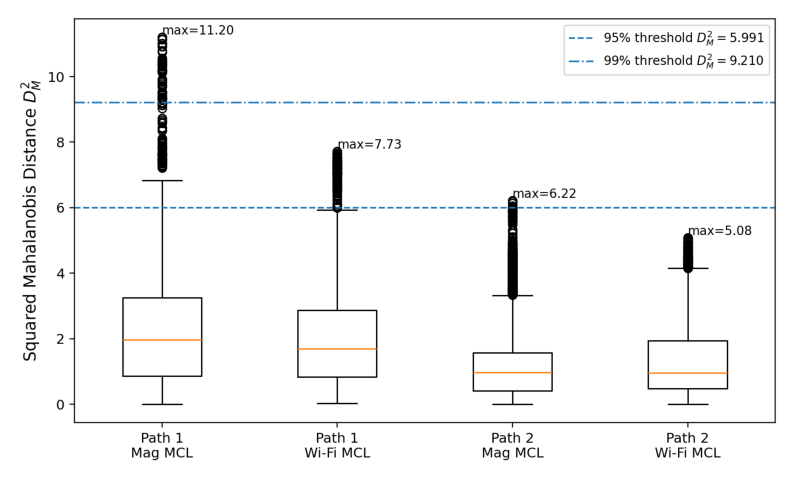
\includegraphics[
    width=0.5\columnwidth
  ]{mahalanobis_full_range_with_max.png}
  \caption{
    Comparison of squared Mahalanobis distance distributions for Mag MCL and Wi-Fi MCL on Path1 and Path2
  }
  \label{fig:mahalanobis_result}
\end{figure}

\begin{table}[t]
  \centering
  \caption{Performance of the LiDAR MCL failure detection on Path 2}
  \label{tab:lidar_failure_detection}
  \scriptsize
  \setlength{\tabcolsep}{4.0pt}
  \renewcommand{\arraystretch}{1.08}
  \small

  \begin{tabular}{lrrr}
    \toprule
    Detection criterion &
    Recall [\%] &
    Precision [\%] &
    FPR [\%] \\
    \midrule
    LiDAR likelihood
      & 91.08 & 86.63 & 32.15 \\
    Particle spread
      & 99.79 & 85.79 & 37.81 \\
    Wi-Fi and Mag ellipses
      & 74.38 & 100.00 & 0.00 \\
    Wi-Fi likelihood
      & 68.83 & 99.29 & 1.12 \\
    \midrule
    Pose Selector
      & 100.00 & 84.97 & 40.48 \\
    \bottomrule
  \end{tabular}
\end{table}


\section{おわりに}
本稿では，磁気強度およびWi-Fi電波強度を用いた不可視地図に基づく自己位置推定と，
不可視地図とLiDARを統合した自己位置推定手法を提案した．
実験の結果，磁気およびWi-Fiを用いた自己位置推定の精度が向上し，
幾何情報が変化した環境においても提案手法が有効であることを確認した．
さらに，LiDAR MCLの位置推定失敗を検知し，
自己位置推定手法を動的に切り替えるシステムを構築し，
その有効性を示した．
今後は，LiDAR MCLの位置推定復帰手法を構築するとともに，
オドメトリの変化を伴わない誘拐状態の検知および復帰を可能とする
自己位置推定システムの実現を目指す．
